

\chapter{Some Group Theory}

Group is a highlight of our course, which interwises topology and algebra. I assume that most students have learnt abstract algebra course MAT3004, and encourage those without this knowledge to read the notes for group posted on blackboard.

\section*{10.6. Wednesday for MAT4002}

\section*{10.6.1. Reviewing On Groups}

\begin{itemize}
\item Example 10.4 Let \({D}_{2n}\) be the regular polygon \(P\) with \({2n}\) sides in \({\mathbb{R}}^{2}\) , centered at the origin. It’s clear that \({D}_{2n}\) is invariant with \({2n}\) rotations, or with 2 reflections. Let \(a\) denote the rotation of \({D}_{2n}\) clockwise by degree \(\pi /n\) , and \(b\) denote the reflection over lines through the origin.
\end{itemize}

As a result, \(\left\{  {e,a,{a}^{2},\ldots ,{a}^{n - 1}}\right\}\) forms a group; and \(\{ e,b\}\) forms a group.

Therefore, all elements of \({D}_{g}\) can be obtained by \({a}^{i}{b}^{j},0 \leq  i \leq  3,0 \leq  j \leq  1\) .

Any finite operations of rotation (the rotation degree is a multiple of \(\pi /n\) ) and reflection can be represented as \({a}^{i}{b}^{j}\) .

Geometrically, we can check that \({ba} = {a}^{n - 1}b\) .

Definition 10.7 [Product Group] Let \(G,H\) be two groups. The product group \(\left( {G \times  H, * }\right)\) is defined as

\[
G \times  H = \{ \left( {g,h}\right)  \mid  g \in  G,h \in  H\}
\]

\[
\text{ with }\left( {{g}_{1},{h}_{1}}\right)  * \left( {{g}_{2},{h}_{2}}\right)  = \left( {{g}_{1}{g}_{2},{h}_{1}{h}_{2}}\right)
\]

For example, \(\left( {\mathbb{R} \times  \mathbb{R}, + }\right)  = \{ \left( {x,y}\right)  \mid  x,y \in  \mathbb{R}\}\) coincides with the usual \({\mathbb{R}}^{2}\) , where

\[
\left( {x,y}\right)  * \left( {{x}^{\prime },{y}^{\prime }}\right)  = \left( {x + {x}^{\prime },y + {y}^{\prime }}\right)
\]

Definition 10.8 A map between two groups \(\phi  : G \rightarrow  H\) is a homomorphism if

\[
\phi \left( {{g}_{1} * {g}_{2}}\right)  = \phi \left( {g}_{1}\right)  * \phi \left( {g}_{2}\right)
\]

In other words, a homomorphism is a map preserving multiplications of groups.

Follow the similar idea as in MAT3040 knowledge, if \(\phi  : G \rightarrow  H\) is a homomorphism, then \(\phi \left( {e}_{G}\right)  = {e}_{H}\) .

\begin{itemize}
\item Example 10.5 Let \(G = \left( {\mathbb{R},+,0}\right)\) , and \(H = \left\{  {{H}_{2},*,{I}_{2}}\right\}\) , with \({H}_{2}\) of the form
\end{itemize}

\[
{H}_{2} = \left\{  {\left. \left( \begin{array}{ll} 1 & x \\  0 & 1 \end{array}\right) \right| \;x \in  \mathbb{R}}\right\}
\]

Define a mapping

\[
\phi  : \;G \rightarrow  H
\]

\[
\text{ with }x \mapsto  \left( \begin{array}{ll} 1 & x \\  0 & 1 \end{array}\right)
\]

Then \(\phi\) is a homorphism:

\[
\phi \left( {x{ * }_{\mathbb{R}}y}\right)  = \phi \left( {x + y}\right)
\]

\[
= \left( \begin{matrix} 1 & x + y \\  0 & 1 \end{matrix}\right)
\]

\[
= \left( \begin{array}{ll} 1 & x \\  0 & 1 \end{array}\right) \left( \begin{array}{ll} 1 & y \\  0 & 1 \end{array}\right)
\]

\[
= \phi \left( x\right)  * {H}_{2}\phi \left( y\right)
\]

Definition 10.9 [Isomorphism] A homomorphism \(\phi  : G \rightarrow  H\) is an isomorphism if \(\phi\) is bijective. The isomorphism between \(G\) and \(H\) is denoted as \(G \cong  H\) .

Actually, a group can be represented as a Cayley Table:

\begin{center}
\adjustbox{max width=\textwidth}{
\begin{tabular}{|c|c|c|c|c|c|}
\hline
\multirow{5}{*}{\(G =\)} & 0 & \({g}_{1}\) & \({g}_{2}\) & ... & \({g}_{n}\) \\
\cline{2-6}
 & \({g}_{1}\) & \({g}_{1} \circ  {g}_{1}\) & \({g}_{1} \circ  {g}_{2}\) & ... & \({g}_{1} \circ  {g}_{n}\) \\
\cline{2-6}
 & \({g}_{2}\) & \({g}_{2} \circ  {g}_{1}\) & \({g}_{2} \circ  {g}_{2}\) & ... & \({g}_{2} \circ  {g}_{n}\) / \\
\cline{2-6}
 & \(\vdots\) & \(\vdots\) & ... & \(\vdots\) & \(\vdots\) \\
\cline{2-6}
 & \({g}_{n}\) & \({g}_{n} \circ  {g}_{1}\) & \({g}_{n} \circ  {g}_{2}\) & ... & \({g}_{n} \circ  {g}_{n}\) \\
\cline{1-6}
\hline
\end{tabular}
}
\end{center}

\begin{center}
\adjustbox{max width=\textwidth}{
\begin{tabular}{|c|c|c|c|c|c|}
\hline
\multirow{5}{*}{\(H =\)} & 0 & \({h}_{1}\) & \({h}_{2}\) & ... & \({h}_{n}\) \\
\cline{2-6}
 & \({h}_{1}\) & \({h}_{1} \circ  {h}_{1}\) & \({h}_{1} \circ  {h}_{2}\) & ... & \({h}_{1} \circ  {h}_{n}\) \\
\cline{2-6}
 & \({h}_{2}\) & \({h}_{2} \circ  {h}_{1}\) & \({h}_{2} \circ  {h}_{2}\) & ... & \({h}_{2} \circ  {h}_{n}\) \\
\cline{2-6}
 & \(\vdots\) & \(\vdots\) & ... & \(\vdots\) & \(\vdots\) \\
\cline{2-6}
 & \({h}_{n}\) & \({h}_{n} \circ  {h}_{1}\) & \({h}_{n} \circ  {h}_{2}\) & ... & \({h}_{n} \circ  {h}_{n}\) \\
\cline{1-6}
\hline
\end{tabular}
}
\end{center}

The groups \(G \cong  H\) if and only if we can find a bijective \(\phi  : G \rightarrow  H\) such that, the Cayley

Table of \(\left( {H, \circ  }\right)\) can be generated from the Cayley Table of \(\left( {G, \circ  }\right)\) by replacing each entry of \(G\) with its image under \(\phi\) .

\section*{10.6.2. Free Groups}

10.10 . Let \(S\) be a (finite) set, which is considered as an "alphabet".

\begin{itemize}
\item Define another set \({S}^{-1} \mathrel{\text{ := }} \left\{  {{x}^{-1} \in  x \in  S}\right\}\) . We insist that \(S \cap  {S}^{-1} = \varnothing\) .
\end{itemize}

\begin{itemize}
\item A word in \(S\) is a finite sequence \(w = {w}_{1}\cdots {w}_{m}\) , where \(m \in  {\mathbb{N}}^{ + } \cup  \{ 0\}\) , and each \({w}_{i} =  \in   \cup  {S}^{-1}\) . In particular, when \(m = 0\) , we view \(w\) as the empty sequence, denoted as \(\varnothing\) .
\end{itemize}

\begin{itemize}
\item The concatenation of two words \({x}_{1}\cdots {x}_{m}\) and \({y}_{1}\cdots {y}_{n}\) is the word \({x}_{1}\cdots {x}_{m}{y}_{1}\cdots {y}_{n}\)
\end{itemize}

\begin{itemize}
\item Two words \(w,{w}^{\prime }\) are equivalent, denoted as \(w \sim  {w}^{\prime }\) , if there are words \({w}_{1},\ldots ,{w}_{n}\) and \(w = {w}_{1},{w}^{\prime } = {w}_{n}\) such that
\end{itemize}

\[
{w}_{i} = \cdots {y}_{1}x{x}^{-1}{y}_{2}\cdots ,\;{w}_{i + 1} = \cdots {y}_{1}{y}_{2}\cdots
\]

or

\[
{w}_{i} = \cdots {y}_{1}{y}_{2}\cdots ,\;{w}_{i + 1} = \cdots {y}_{1}x{x}^{-1}{y}_{2}\cdots
\]

for some \(x \in  S \cup  {S}^{-1}\) .

\begin{itemize}
\item Example 10.6 For example, \(S = \{ a,b\}\) and \({S}^{-1} = \left\{  {{a}^{-1}{b}^{-1}}\right\}\) and
\end{itemize}

\[
w = {aaba}{b}^{-1}{b}^{-1}{a}^{-1}{abaab}{b}^{-1}a
\]

\[
{w}^{\prime } = {aaba}{b}^{-1}{b}^{-1}{a}^{-1}{abaaa}
\]

Here \(w\) and \({w}^{\prime }\) differs by \(b{b}^{-1}\) . Therefore, \(w \sim  {w}^{\prime }\) , and \(w\) is said to be a elementary expansion of \({w}^{\prime }\) .

We insist that \({\left( {s}^{-1}\right) }^{-1} = s,\forall {s}^{-1} \in  {S}^{-1}\) , since otherwise for \(x = {s}^{-1} \in  {S}^{-1}\) , we cannot define \({\left( {s}^{-1}\right) }^{-1}\) .

Moreover, for

\[
w = {aaba}{b}^{-1}{b}^{-1}{a}^{-1}{abaab}{b}^{-1}a
\]

\[
{w}^{\prime \prime } = {aaba}{b}^{-1}{b}^{-1}{baab}{b}^{-1}a,
\]

\(w\) and \({w}^{\prime \prime }\) differs by \({a}^{-1}a\) , i.e., \({a}^{-1}{\left( {a}^{-1}\right) }^{-1}\) , and therefore \(w \sim  {w}^{\prime \prime }\) .

Definition 10.11 [Free Group] The free group \(F\left( S\right)\) is defined to be the equivalence class of words, i.e.,

\[
\left\lbrack  w\right\rbrack   \mathrel{\text{ := }} \left\{  {{w}^{\prime }\text{ is a word in }S \mid  w \sim  {w}^{\prime }}\right\}   \in  F\left( S\right)
\]

\(F\left( S\right)\) is indeed a group:

\begin{itemize}
\item \(\left\lbrack  w\right\rbrack   * \left\lbrack  {w}^{\prime }\right\rbrack   = \left\lbrack  {w{w}^{\prime }}\right\rbrack\) (concatenation) check \({w}_{1} \sim  {w}_{2},{u}_{1} \sim  {u}_{2}\) implies \({w}_{1}{u}_{1} \sim\)  \({w}_{2}{u}_{2}\)
\end{itemize}

\begin{itemize}
\item Identity element: \(e = \left\lbrack  \varnothing \right\rbrack\)
\end{itemize}

\begin{itemize}
\item Inverse element: \({\left\lbrack  {x}_{1}\cdots {x}_{n}\right\rbrack  }^{-1} = \left\lbrack  {{x}_{n}^{-1}\cdots {x}_{1}^{-1}}\right\rbrack\)
\end{itemize}

\begin{itemize}
\item Example 10.7 Let \(S = \{ a\}\) and \({S}^{-1} = \left\{  {a}^{-1}\right\}\) . Any word \(w\) has the form
\end{itemize}

\[
w = a\cdots a{a}^{-1}\cdots {a}^{-1}a\cdots a{a}^{-1}\cdots {a}^{-1}\cdots
\]

In shorthand, we denote \(w\) as \(w = \cdots {a}^{p}{\left( {a}^{-1}\right) }^{q}{a}^{r}{\left( {a}^{-1}\right) }^{s}\cdots\) , and

\[
\left\lbrack  w\right\rbrack   = \left\lbrack  {\cdots {a}^{p}{\left( {a}^{-1}\right) }^{q}{a}^{r}{\left( {a}^{-1}\right) }^{s}\cdots }\right\rbrack   = \left\lbrack  {\cdots {a}^{p - 1}{\left( {a}^{-1}\right) }^{q - 1}{a}^{r}{\left( {a}^{-1}\right) }^{s}\cdots }\right\rbrack
\]

\[
= \left\lbrack  {\cdots {a}^{p - 1}{\left( {a}^{-1}\right) }^{q - 2}{a}^{r - 1}{\left( {a}^{-1}\right) }^{s}\cdots }\right\rbrack  ,
\]

e.g., we can always eliminate the adjacent terms \(a\) and \({a}^{-1}\) up to equivalence class. Therefore, \(F\left( S\right)  = \left\{  {\cdots ,\left\lbrack  {a}^{-2}\right\rbrack  ,\left\lbrack  {a}^{-1}\right\rbrack  ,\left\lbrack  \varnothing \right\rbrack  ,\left\lbrack  a\right\rbrack  ,\left\lbrack  {a}^{2}\right\rbrack  ,\cdots }\right\}\) .

It’s clear that \(F\left( S\right)  \cong  \mathbb{Z}\) , where the isomorphism \(\phi  : \mathbb{Z} \rightarrow  F\left( S\right)\) is \(\phi \left( n\right)  = \left\lbrack  {a}^{n}\right\rbrack\) .

\begin{itemize}
\item Example 10.8 Let \(S = \{ a,b\}\) and \({S}^{-1} = \left\{  {{a}^{-1},{b}^{-1}}\right\}\) . In this case, \(\left\lbrack  {ab}\right\rbrack   \neq  \left\lbrack  {ba}\right\rbrack\) , and \(\left\lbrack  {a{b}^{-1}{a}^{2}{b}^{2}{a}^{-2}b}\right\rbrack\) cannot be reduced further.
\end{itemize}

Since \(S\) is not an abelian group in such case, we imply \(F\left( S\right)  ≆ \mathbb{Z} \times  \mathbb{Z}\) .

\section*{10.6.3. Relations on Free Groups}

Definition 10.12 [Group With Relations] Let \(S\) be a set. A group with relations is written as

\[
G = \langle S \mid  R\left( S\right) \rangle
\]

where

\begin{itemize}
\item \(R\left( S\right)\) consists of elements in \(F\left( S\right)\)
\end{itemize}

\begin{itemize}
\item Every element in \(G\) can be written as the form \(\left\lbrack  w\right\rbrack   \in  F\left( S\right)\) , and we insist that \(\left\lbrack  w\right\rbrack   = \left\lbrack  {w}^{\prime }\right\rbrack\) in \(G\) if
\end{itemize}

\begin{itemize}
\item \(w\) and \({w}^{\prime }\) differ by some \(x{x}^{-1},x \in  S \cup  {S}^{-1}\) , or
\end{itemize}

\begin{itemize}
\item \(w\) and \({w}^{\prime }\) differ by some element \(z \in  R\left( S\right)\) , or its inverse.
\end{itemize}

\begin{itemize}
\item Example 10.9 Let \(G = \left\langle  {a,b \mid  {a}^{2},{b}^{2},{aba}{b}^{-1}{a}^{-1}{b}^{-1}}\right\rangle\) , we want to enumerate all possible elements in \(G\) . Obseve that
\end{itemize}

\[
\left\lbrack  {b}^{-1}\right\rbrack   = \left\lbrack  {{b}^{-1}{b}^{2}}\right\rbrack   = \left\lbrack  b\right\rbrack  ,\;\text{ similarly }\left\lbrack  {a}^{-1}\right\rbrack   = \left\lbrack  a\right\rbrack
\]

\[
\left\lbrack  {bab}\right\rbrack   = \left\lbrack  {{aba}{b}^{-1}{a}^{-1}{b}^{-1}{bab}}\right\rbrack   = \left\lbrack  {{aba}{b}^{-1}b}\right\rbrack   = \left\lbrack  {aba}\right\rbrack
\]

As a result,

\begin{itemize}
\item \(\left\lbrack  {a}^{-n}\right\rbrack   = \left\lbrack  {a}^{n}\right\rbrack\) and \(\left\lbrack  {b}^{-n}\right\rbrack   = \left\lbrack  {b}^{n}\right\rbrack\)
\end{itemize}

\begin{itemize}
\item \(\left\lbrack  {a}^{{2n} + 1}\right\rbrack   = \left\lbrack  a\right\rbrack  ,\left\lbrack  {b}^{{2n} + 1}\right\rbrack   = \left\lbrack  b\right\rbrack  ,\left\lbrack  {a}^{2n}\right\rbrack   = \left\lbrack  \varnothing \right\rbrack  ,\left\lbrack  {b}^{2n}\right\rbrack   = \left\lbrack  \varnothing \right\rbrack\)
\end{itemize}

\begin{itemize}
\item For another type of element of \(G\) , it must be of the form \(\left\lbrack  {\cdot {abababab}\cdots }\right\rbrack\) .
\end{itemize}

Each aba can be changed into \({bab}\) , and finally it will be reduced into the form \(\left\lbrack  {ab}\right\rbrack\) . Therefore, the elements in \(G\) are

\[
\left\lbrack  \varnothing \right\rbrack  ,\left\lbrack  a\right\rbrack  ,\left\lbrack  b\right\rbrack  ,\left\lbrack  {ab}\right\rbrack  ,\left\lbrack  {ba}\right\rbrack  ,\left\lbrack  {aba}\right\rbrack
\]

In fact, \(G \cong  {S}_{3}\) .

\section*{11.3. Monday for MAT4002}

Reviewing. Consider the group with presentation \(\langle S \mid  R\left( S\right) \rangle\) .

1. The elements in \(S\) are generators that have studied in abstract algebra

2. The "relations" of this group are given by the equalities on hte right-hand side, e.g., the dihedral group is defined as

\[
\left\langle  {a,b \mid  {a}^{n} = e,{b}^{2} = e,{bab} = {a}^{-1}}\right\rangle
\]

Sometimes we also simplify the equality \(\times   = e\) as \(\times\) , e.g., the dihedral group can be re-written as

\[
\left\langle  {a,b \mid  {a}^{n},{b}^{2},{bab} = {a}^{-1}}\right\rangle
\]

\section*{Example 11.4 Consider}

\[
G =  < a,b \mid  {a}^{2},{b}^{2},{aba}{b}^{-1}{a}^{-1}{b}^{-1} >  \mathrel{\text{ := }}  < a,b \mid  {a}^{2},{b}^{2},{aba} = {bab} >  = \{ e,a,b,{ab},{ba},{aba}\}
\]

It’s isomorphic to \({S}^{3}\) , and the shape of \({S}^{3}\) is illustrated in Fig.(11.1)

\begin{center}
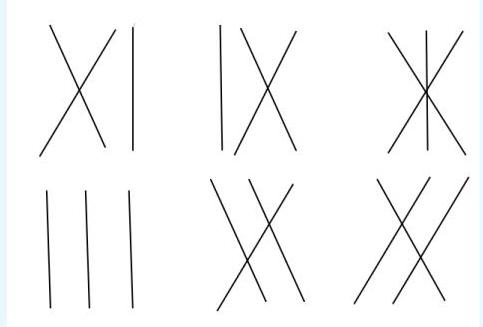
\includegraphics[max width=0.4\textwidth]{images/bo_d2bcsrref24c73avs720_107_737_1365_483_327_0.jpg}
\end{center}
\hspace*{3em} 

Figure 11.1: Illustration of group \({S}^{3}\)

More precisely, the isomorphism is given by:

\[
\phi  : \;{S}_{3} \rightarrow  G
\]

\[
\text{ with }X \mid   \mapsto  a,\; \mid  X \mapsto  b
\]

\begin{itemize}
\item Example 11.5 Consider \({G}_{2} =  < a,b \mid  {ab} = {ba} >\) and any word, which can be expressed as \(\cdots {a}^{s}{b}^{t}{a}^{u}{b}^{v}\cdots\)
\end{itemize}

\begin{itemize}
\item If \(s \in  \mathbb{N}\) , we write \({a}^{s} \mathrel{\text{ := }} \underset{s\text{ times }}{\underbrace{a\cdots a}}\)
\end{itemize}

\begin{itemize}
\item If \(s \in   - \mathbb{N}\) , we write \({a}^{s} \mathrel{\text{ := }} \underset{-s\text{ times }}{\underbrace{\left( {a}^{-1}\right) \cdots \left( {a}^{-1}\right) }}\)
\end{itemize}

\begin{itemize}
\item For the word with the form \(a\cdots b\cdots {ba}\cdots a\) , we can always push \(a\) into the leftmost using the relation \({ab} = {ba}\)
\end{itemize}

\begin{itemize}
\item For the word with the form \(a\cdots {ab}\cdots b{a}^{-1}\) , we can always push \({a}^{-1}\) into the leftmost using the relation \(b{a}^{-1} = {a}^{-1}b\) .
\end{itemize}

Therefore, all elements in \({G}_{2}\) are of the form \({a}^{p}{b}^{q},p,q \in  \mathbb{Z}\) , and we have the relation

\[
\left( {{a}^{{p}_{1}}{b}^{{q}_{1}}}\right) \left( {{a}^{{p}_{2}}{b}^{{q}_{2}}}\right)  = {a}^{{p}_{1} + {p}_{2}}{b}^{{q}_{1} + {q}_{2}}.
\]

Therefore, \({G}_{2} \cong  \mathbb{Z} \times  \mathbb{Z}\) , where the isomorphism is given by:

\[
\phi  : \;\mathbb{Z} \times  \mathbb{Z} \rightarrow  {G}_{2}
\]

\[
\text{ with }\left( {p,q}\right)  \mapsto  {a}^{p}{b}^{q}
\]

\begin{itemize}
\item Example 11.6
\end{itemize}

\[
{G}_{3} = \left\langle  {a \mid  {a}^{5}}\right\rangle   = \left\{  {1,a,{a}^{2},\ldots ,{a}^{4}}\right\}
\]

It’s clear that \({G}_{3} \cong  \mathbb{Z}/5\mathbb{Z}\) , where the isomorphism is given by:

\[
\phi  : \;\mathbb{Z}/5\mathbb{Z} \rightarrow  {G}_{3}
\]

\[
\text{ with }m + 5\mathbb{Z} \mapsto  {a}^{m}
\]

\section*{11.3.1. Cayley Graph for finitely presented groups}

Graphs have strong connection with groups. Here we introduce a way of building graphs using groups, and the graphs are known as Cayley graphs. They describe many properties of the group in a topological way.

Definition 11.5 [Oriented Graph] An oriented graph \(T\) is specified by

1. A countable or finite set \(V\) , known as vertices

2. A countable or finite set \(E\) , known as edges

3. A function \(\delta  : E \rightarrow  V \times  V\) given by

\[
\delta \left( e\right)  = \left( {\ell \left( e\right) ,\tau \left( e\right) }\right)
\]

where \(\ell \left( e\right)\) denotes the initial vertex and \(\tau \left( e\right)\) denotes the terminal vertex.

For example, let

\begin{itemize}
\item \(V = \{ a,b,c\}\)
\end{itemize}

\begin{itemize}
\item \(E = \left\{  {{e}_{1},{e}_{2},{e}_{3},{e}_{4}}\right\}\)
\end{itemize}

\begin{itemize}
\item \(\delta \left( {e}_{1}\right)  = \left( {a,a}\right) ,\delta \left( {e}_{2}\right)  = \left( {b,c}\right) ,\delta \left( {e}_{3}\right)  = \left( {a,c}\right) ,\delta \left( {e}_{4}\right)  = \left( {b,c}\right)\)
\end{itemize}

\begin{center}
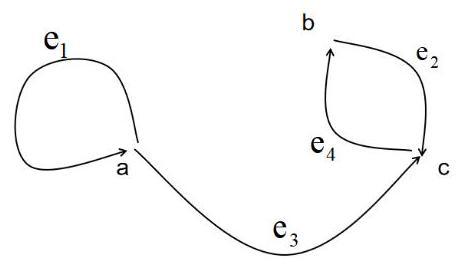
\includegraphics[max width=0.3\textwidth]{images/bo_d2bcsrref24c73avs720_109_740_1525_457_264_0.jpg}
\end{center}
\hspace*{3em} 

Figure 11.2: Illustration of example oriented graph

The resulted graph is plotted in Fig.(11.2)

Definition 11.6 [Cayley graph] Let \(G = \langle S \mid  R\left( S\right) \rangle\) with \(\left| S\right|  < \infty\) . The Cayley graph associated to \(G\) is an oriented graph with

1. The vertex set \(G\)

2. The edge set \(E \mathrel{\text{ := }} G \times  S\)

3. The function \(\ell  : E \rightarrow  V \times  V\) is given by:

\(\ell  : \;G \times  S \rightarrow  G \times  G\)

with \(\left( {g,s}\right)  \mapsto  \left( {g,g \cdot  s}\right)\)

In particular, we link two elements in \(G\) if they differ by a generator rightside.

1. The Cayley graph for \(G = \langle a\rangle \left( { \cong  \mathbb{Z}}\right)\) is shown in Fig.(11.3):

\begin{center}
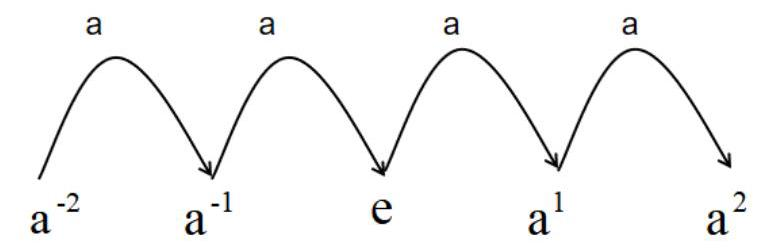
\includegraphics[max width=0.6\textwidth]{images/bo_d2bcsrref24c73avs720_110_448_1055_769_250_0.jpg}
\end{center}
\hspace*{3em} 

Figure 11.3: Illustration of Cayley Graph \(\langle a\rangle\)

2. The Cayley graph for \(G = \left\langle  {a \mid  {a}^{3}}\right\rangle\) is shown in Fig.(11.4):

\begin{center}
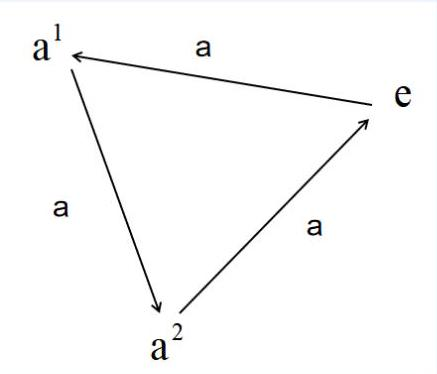
\includegraphics[max width=0.3\textwidth]{images/bo_d2bcsrref24c73avs720_110_618_1541_437_374_0.jpg}
\end{center}
\hspace*{3em} 

Figure 11.4: Illustration of Cayley Graph \(\left\langle  {a \mid  {a}^{3}}\right\rangle\)

3. The Cayley graph for \(G = \left\langle  {a,b \mid  {a}^{2},{b}^{2},{aba} = {bab}}\right\rangle\) is shown in Fig.(11.12):

\begin{center}
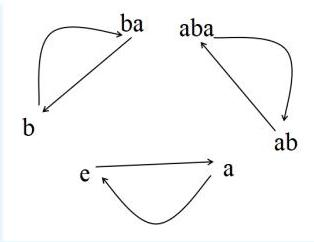
\includegraphics[max width=0.2\textwidth]{images/bo_d2bcsrref24c73avs720_111_811_303_314_242_0.jpg}
\end{center}
\hspace*{3em} 

Figure 11.5: Illustration of Cayley Graph \(\left\langle  {a,b \mid  {a}^{2},{b}^{2},{aba} = {bab}}\right\rangle\)

4. The Cayley graph for \(G = \langle a,b \mid  {ab} = {ba}\rangle\) is shown in Fig.(11.6):

\begin{center}
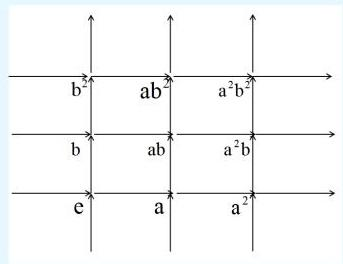
\includegraphics[max width=0.2\textwidth]{images/bo_d2bcsrref24c73avs720_111_805_742_343_264_0.jpg}
\end{center}
\hspace*{3em} 

Figure 11.6: Illustration of Cayley Graph \(\langle a,b \mid  {ab} = {ba}\rangle\)

5. The Cayley graph for \(G = \langle a,b\rangle\) is shown in Fig.(11.7):

\begin{center}
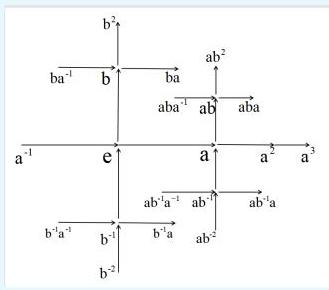
\includegraphics[max width=0.2\textwidth]{images/bo_d2bcsrref24c73avs720_111_809_1204_329_290_0.jpg}
\end{center}
\hspace*{3em} 

Figure 11.7: Illustration of Cayley Graph \(\langle a,b \mid  {ab} = {ba}\rangle\)

There could be different presentations \(\left\langle  {{S}_{1} \mid  R\left( {S}_{1}\right) }\right\rangle   \cong  \left\langle  {{S}_{2} \mid  R\left( {S}_{2}\right) }\right\rangle\) of the same group.